\documentclass[twocolumn]{aastex701}

\newcommand{\rade}{R_\oplus}
\newcommand{\msun}{M_\odot}
\newcommand{\slope}{m}

\begin{document}

\title{Revisiting the Slope of the M-dwarf Radius Valley with the 2026 Confirmed-Planet Catalog}

\author{Cho Seunghyeon}
\affiliation{Undergraduate research project}
\email{[email protected]}

\begin{abstract}
The radius valley separating super-Earths from sub-Neptunes provides a
sensitive test of planet formation and evolution, but its behavior around
M dwarfs remains debated: published slopes ($\slope = d\log R_p/d\log P$)
disagree in sign, and the valley may vanish entirely at the lowest stellar
masses. Using the NASA Exoplanet Archive (accessed 2026 July), we construct
stellar-mass subsamples of transiting planets and characterize the radius
distribution with complementary statistics: a bootstrapped gap-depth measure,
Hartigan's dip test with power simulations, a super-Earth to sub-Neptune count
ratio, and two independent slope estimators (a rotating-band density scan and
a support-vector-machine boundary fit). We recover the valley in K- and
G-type control samples with slopes consistent with published values,
validating the pipeline. Around mid-to-late M dwarfs
($M_\star < 0.4~\msun$) the radius distribution is unimodal and robust to
radius-precision cuts, with super-Earths outnumbering sub-Neptunes. For the
combined M-dwarf sample the two estimators return negative slopes
($\slope = -0.13$ and $-0.16$) when the fit is confined to the physically
plausible valley region, favoring the mass-loss sign, although the
uncertainties do not exclude a positive slope at 95\% confidence. We further
show that an unconstrained gap search instead locks onto the
detection-completeness boundary, demonstrating that methodological choices can
flip the inferred sign. We suggest this sensitivity contributes to the
literature disagreement.
\end{abstract}

%% ============================================================
%% 서론(Introduction)은 마지막에 추가 예정.
%% 아래: 데이터(Data) + 방법(Methods) + 결과(Results).
%% ============================================================

\section{Introduction} \label{sec:intro}

The distribution of small-planet radii contains a narrow deficit near
$1.5$--$2.0~\rade$, the radius valley, that separates rocky super-Earths from
gas-enveloped sub-Neptunes \citep{Fulton2017}. Because a planet's size reflects
whether it has retained a hydrogen-helium envelope, the valley is a direct
observational probe of planet formation and evolution. Its discovery was
enabled by improved stellar radii---first from spectroscopy and subsequently
from Gaia parallaxes---which sharpened planetary radii enough to resolve the
feature \citep{Fulton2018}. The valley is not a fixed radius but shifts with
orbital period: around FGK stars it moves to smaller radii at longer period,
with a slope $\slope \equiv d\log R_p/d\log P \approx -0.11$
\citep{VanEylen2018}.

The sign of this slope discriminates between formation scenarios. Thermally
driven atmospheric mass loss---whether photoevaporation by stellar high-energy
radiation \citep{OwenWu2017} or core-powered mass loss---predicts a negative
slope, because planets closer to the star are stripped to larger core radii. A
positive slope would instead point to a valley established at formation in a
gas-poor inner disk, without the need for subsequent stripping. Around
Sun-like stars the observed negative slope is consistent with the mass-loss
picture, although the negative sign alone does not distinguish photoevaporation
from core-powered mass loss.

Whether the same picture holds around M dwarfs, the most common stars in the
Galaxy, remains contested. \citet{Cloutier2020} measured a \emph{positive}
slope of $+0.058 \pm 0.022$ for planets around low-mass stars, opposite in sign
to the FGK trend, and interpreted it as evidence for an increasing role of
gas-poor formation at low stellar mass. In contrast, \citet{VanEylen2021},
using a support-vector-machine boundary fit, found a \emph{negative} slope near
$-0.11$ for M-dwarf planets, consistent with the FGK trend and with mass loss.
More recent work suggests the valley may become shallow or disappear entirely
toward the lowest stellar masses, leaving the radius distribution effectively
unimodal. The disagreement is notable because the studies analyze similar
stellar populations yet reach opposite conclusions, raising the possibility
that sample selection and methodology, rather than a physical difference,
drive the discrepancy.

The number of confirmed transiting planets has grown substantially since these
analyses, offering an opportunity to revisit the question with a larger sample.
In this work we use the 2026 NASA Exoplanet Archive to characterize the
M-dwarf radius distribution and to measure the valley slope with two
independent estimators, validating the pipeline against FGK control samples.
Rather than aiming to settle the debate, we ask which sign the current data
favor and, equally, how strongly the answer depends on analysis choices. We
describe the data in Section~\ref{sec:data}, the methods in
Section~\ref{sec:methods}, our results in Section~\ref{sec:results}, and their
interpretation in Section~\ref{sec:discussion}.

\section{Data} \label{sec:data}

We use the NASA Exoplanet Archive Planetary Systems Composite Parameters
table (\texttt{pscomppars}), which provides one row per planet by combining
literature values, accessed 2026 July. We query for transiting planets
(\texttt{tran\_flag}~$=1$) with non-null planetary radius $R_p$
(\texttt{pl\_rade}), orbital period $P$ (\texttt{pl\_orbper}), and host
stellar mass $M_\star$ (\texttt{st\_mass}). Transit-derived radii and periods
are the two quantities that define the radius valley: the transit depth sets
$R_p/R_\star$, and the interval between transits sets $P$. Because the radius
valley is a narrow feature, the reliability of $R_p$---which inherits the
uncertainty of the adopted stellar radius---is the limiting factor, and we
control for it explicitly below.

We restrict the analysis to $R_p < 4~\rade$ and $P < 100$~d. The upper radius
limit excludes gas giants, which are unrelated to the super-Earth/sub-Neptune
transition, while retaining both flanks of the valley. The period limit
excludes the long-period regime where transit detection is highly incomplete.
For each planet we compute the fractional radius uncertainty as the mean of the
absolute upper and lower errors divided by $R_p$, and adopt an 8\% cut for the
fiducial sample, following the precision regime in which the valley was first
resolved. We partition the sample into stellar-mass bins approximating spectral
type: mid-to-late M ($M_\star < 0.4~\msun$), early M ($0.4$--$0.6$),
K ($0.6$--$0.85$), G ($0.85$--$1.1$), and F ($1.1$--$1.4~\msun$), plus a
combined M-dwarf bin ($M_\star < 0.6~\msun$) used for slope measurement, where
the individual M subsamples are small. These boundaries are approximate and are
tested for sensitivity.

\section{Methods} \label{sec:methods}

\subsection{Distribution Statistics}
\label{sec:methods_dist}

To assess whether a subsample is bimodal we use three complementary
statistics. First, a gap-depth statistic $D = 1 - \rho_{\rm valley} /
\overline{\rho_{\rm peak}}$ compares the number density in a valley window to
the mean density of the two flanking peak windows, where each density is
normalized by the logarithmic width of its window. $D \to 1$ indicates an empty
valley and $D \to 0$ indicates no depletion. Because $D$ presupposes two
populated peaks, we adopt a mass-scaled window centered on the expected valley
location $R_{\rm valley} = 1.86\,(M_\star/\msun)^{0.18}~\rade$
\citep{Petigura2022} and return $D$ as undefined when either flanking window
contains fewer than five planets; this prevents the statistic from measuring
the edge of a unimodal distribution.

Second, we apply Hartigan's dip test to $\log_{10} R_p$, whose null hypothesis
is unimodality. To interpret a non-rejection we estimate the test's power by
generating synthetic bimodal distributions matched to the control-sample size
and measuring the fraction in which the dip test rejects unimodality.

Third, as a statistic that assumes no particular modality, we count planets
below and above the mass-scaled valley line to form a super-Earth to
sub-Neptune ratio. Uncertainties on $D$ and on the ratio are obtained by
bootstrap resampling ($N = 2000$) with a fixed random seed.

\subsection{Slope Estimators}
\label{sec:methods_slope}

We model the valley as $R = R_0\,(P/10~{\rm d})^{\slope}$, a line in the
$\log P$--$\log R$ plane with slope $\slope$ and reference radius $R_0$ at
$P = 10$~d. We measure $\slope$ with two estimators of differing principle.

The rotating-band scan searches a grid in $(\slope, R_0)$ and, for each
candidate line, counts planets within a band of half-width $hw = 0.04$~dex and
compares this to the count in adjacent reference regions; the line maximizing
the deficit relative to its flanks is selected. Grid points whose reference
region is sparsely populated are skipped.

The support-vector-machine (SVM) boundary fit labels planets above and below
an initial mass-scaled dividing line and fits a linear maximum-margin
hyperplane $w_0 \log P + w_1 \log R + b = 0$, from which the slope follows as
$\slope = -w_0/w_1$. Planets are relabeled by the fitted boundary and the fit
is iterated to reduce dependence on the initial labels. We use soft-margin
strength $C = 1$ and balanced class weights in the fiducial configuration.

For both estimators, confidence intervals are obtained by bootstrap resampling
in which period and radius are resampled with the same indices to preserve each
planet's $(P, R)$ pairing. For the M-dwarf sample we additionally restrict to
$P < 30$~d to limit contamination from detection incompleteness at long period.
We validate both estimators on the G and K samples, where the recovered slopes
can be compared to published FGK values.

The hyperparameters above ($hw$, $C$, the mass bin edges, and the initial
dividing line) are analysis choices rather than measured quantities; we
therefore vary each and report the resulting spread in
Section~\ref{sec:sensitivity}. The valley-location scaling
($1.86\,(M_\star/\msun)^{0.18}$) is adopted from the literature
\citep{Petigura2022}, and the random seed and bootstrap count affect only the
stability of the intervals, not the point estimates.

\section{Results} \label{sec:results}

\subsection{The Radius Distribution Is Unimodal Around Low-Mass M Dwarfs}
\label{sec:unimodal}

Figure~\ref{fig:errorcuts} shows the radius distributions of the five
stellar-mass subsamples under three radius-precision cuts. The mid-to-late
M-dwarf sample ($M_\star < 0.4~\msun$) exhibits a single peak near
$1.2~\rade$ that persists across all three cuts, from the full sample down to
planets with radius uncertainties below 8\%. The peak location and unimodal
character are therefore not artifacts of measurement precision. In contrast,
the G and K subsamples develop an increasingly clear bimodal structure as the
precision cut is tightened, with a depletion near $1.8~\rade$ separating the
super-Earth and sub-Neptune populations. The early-M subsample
($0.4$--$0.6~\msun$) is intermediate, showing a partially filled depletion.

\begin{figure*}
\centering
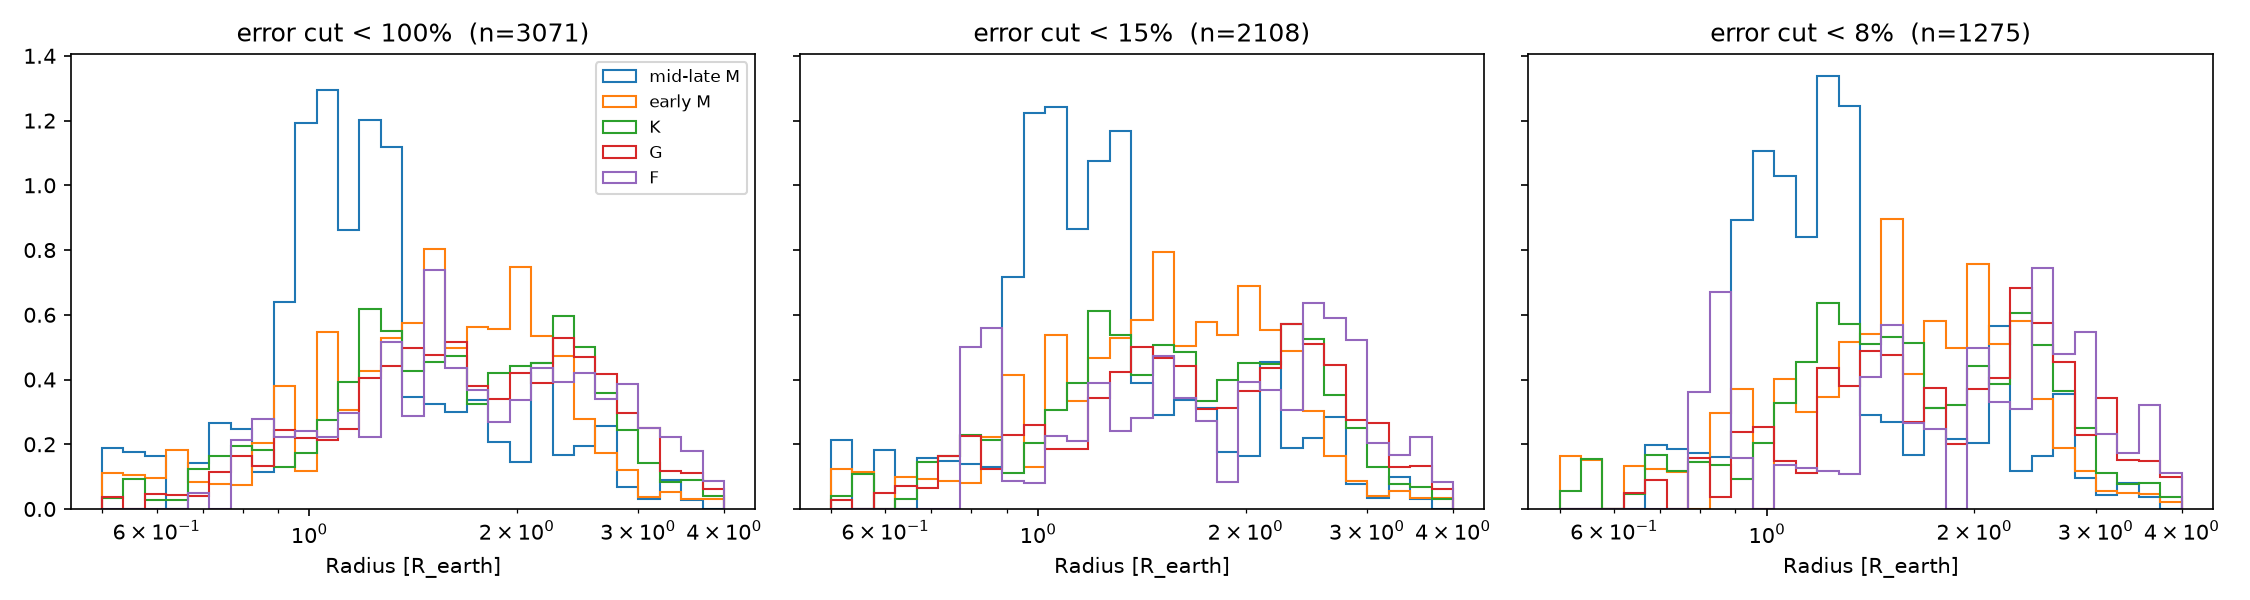
\includegraphics[width=\textwidth]{figures/fig1_error_cuts.png}
\caption{Normalized radius distributions for five stellar-mass subsamples
under radius-precision cuts of 100\%, 15\%, and 8\% (left to right). The
mid-to-late M-dwarf peak near $1.2~\rade$ is stable across cuts, while the
G and K depletion near $1.8~\rade$ sharpens as precision improves.
\label{fig:errorcuts}}
\end{figure*}

\subsection{Failure of One-Dimensional Bimodality Tests}
\label{sec:diptest}

A fixed-window gap-depth statistic $D$ returns a large positive value for the
mid-to-late M sample ($D = 0.41$). Diagnostic counts show that this reflects
the sharp upper edge of a unimodal distribution rather than a true valley:
the putative upper peak window ($2.2$--$2.8~\rade$) contains only 13 planets,
so the statistic measures a cliff, not a gap. When the depth statistic is
restricted to bins in which both flanking peaks are populated, the mid-to-late
M value becomes undefined, consistent with the absence of a valley.

Hartigan's dip test does not reject unimodality for any subsample, including
the G sample in which a valley is visually and statistically evident
(dip $p = 0.97$). A power simulation using synthetic bimodal distributions
matched to the G sample size recovers the injected bimodality in 93\% of
trials. The failure to reject unimodality in real data therefore does not
arise from insufficient statistical power; rather, the one-dimensional test is
degraded because the valley is inclined in the period--radius plane, so that
superposing multiple periods fills the depletion. This motivates a direct
measurement of the valley slope.

\subsection{The Super-Earth to Sub-Neptune Ratio Increases Toward Lower
Stellar Mass}
\label{sec:ratio}

The ratio of super-Earths to sub-Neptunes, defined relative to a
mass-scaled valley location, increases monotonically with decreasing stellar
mass, from $0.39$ (F) and $0.49$ (G) to $0.79$ (K) and $1.49$ for the
mid-to-late M sample (Figure~\ref{fig:ratio}). The mid-to-late M value
exceeds unity at $1.49\,[1.22,\,1.83]$ (68\% confidence). Because this
statistic makes no assumption about the modality of the distribution, it is
not subject to the failure mode of Section~\ref{sec:diptest}. The trend is
consistent with a valley that fades toward low stellar mass. We caution that
these are raw counts without completeness correction; because small planets
are harder to detect, the super-Earth counts are underestimated, so the true
ratios are likely larger, which strengthens rather than weakens the direction
of the trend.

\begin{figure}
\centering
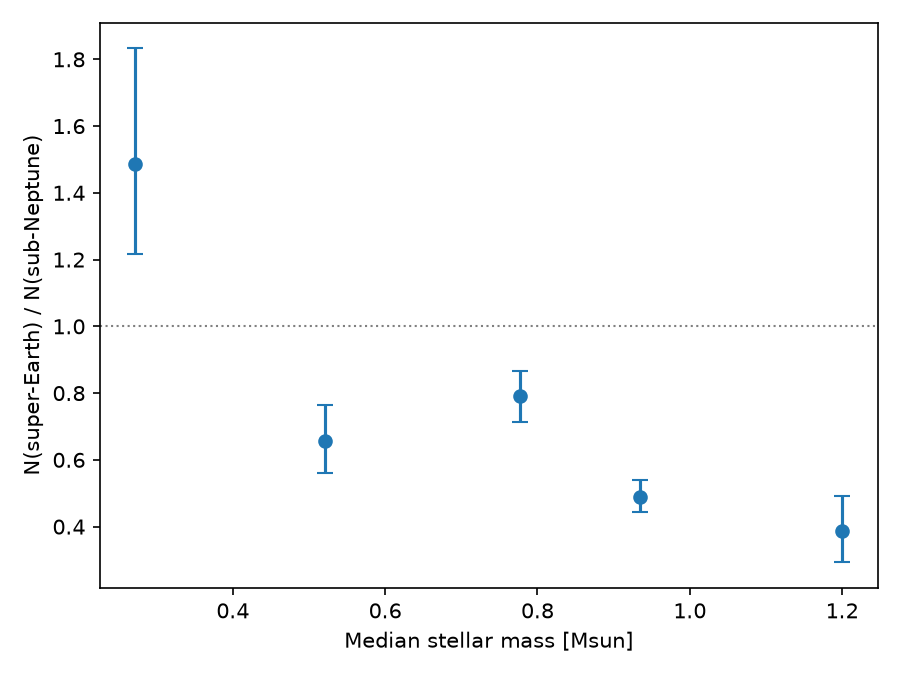
\includegraphics[width=\columnwidth]{figures/fig2_se_sn_ratio.png}
\caption{Super-Earth to sub-Neptune count ratio versus median stellar mass
for each subsample, with 68\% bootstrap intervals. The dotted line marks
parity. The ratio rises toward lower stellar mass and exceeds unity for the
mid-to-late M sample.
\label{fig:ratio}}
\end{figure}

\subsection{Valley Slope: Two Independent Estimators}
\label{sec:slope}

We measure the valley slope with two methods of differing principle. The
rotating-band scan locates the orientation of the band that is most depleted
relative to its flanks; the support-vector-machine (SVM) boundary fit labels
planets above and below a mass-scaled dividing line and finds the maximum-margin
hyperplane separating them. Applied to the G and K control samples, the band scan returns
$\slope = -0.09$ and $-0.07$, respectively. The G-sample value matches the
FGK valley slope of $\slope = -0.09$ reported by \citet{VanEylen2018}, and
both control slopes are consistent in sign and magnitude with published FGK
measurements near $-0.11$, validating the pipeline.

For the combined M-dwarf sample ($M_\star < 0.6~\msun$; period restricted to
$P < 30$~d to mitigate incompleteness), the band scan returns
$\slope = -0.13$ (95\% CI $[-0.23,\,+0.07]$) and the SVM boundary returns
$\slope = -0.16$ (95\% CI $[-0.28,\,-0.02]$) in its fiducial configuration,
with a boundary radius of $1.46~\rade$ consistent with the expected valley
location. Both point estimates favor the negative, mass-loss sign, and the
fiducial SVM interval excludes both zero and the previously reported positive
value ($+0.058$). Our SVM slope is furthermore consistent with the
$\slope \approx -0.11$ obtained by \citet{VanEylen2021} using the same
boundary-fitting technique on an independent M-dwarf sample. Figure~\ref{fig:overlay} shows the two fitted loci
overlaid on the M-dwarf sample.

\begin{figure}
\centering
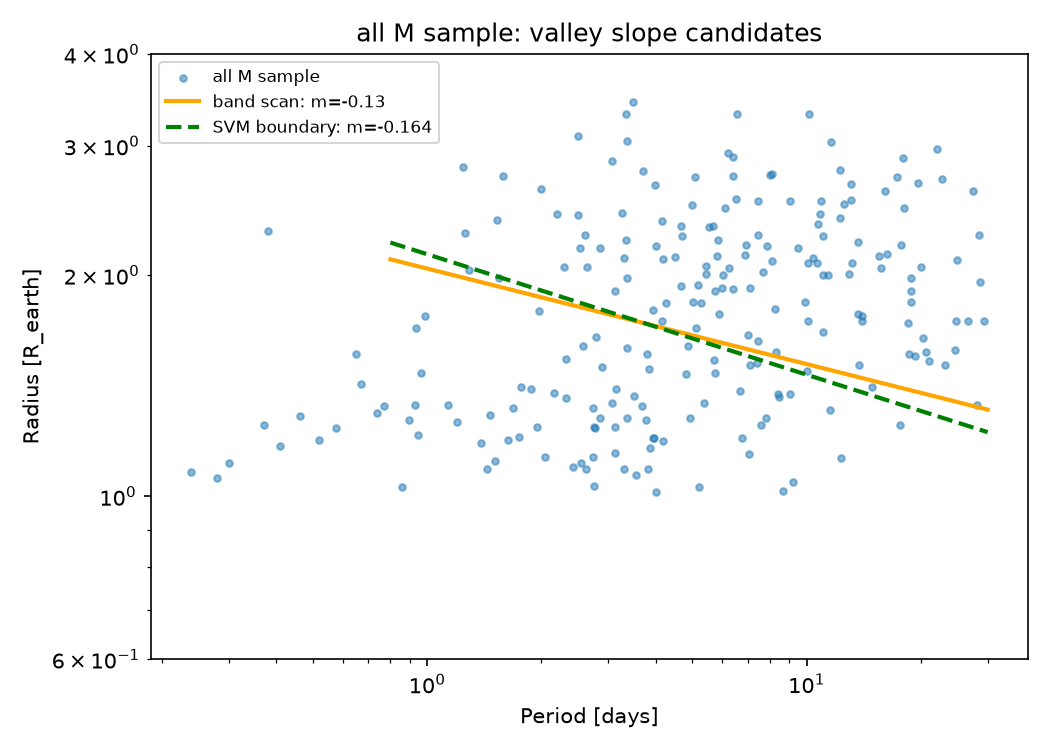
\includegraphics[width=\columnwidth]{figures/fig3_slope_overlay.png}
\caption{Period--radius distribution of the combined M-dwarf sample with the
valley loci from the band scan (solid) and the SVM boundary (dashed). The two
independent estimators return consistent negative slopes.
\label{fig:overlay}}
\end{figure}

\subsection{Sensitivity to Methodological Choices}
\label{sec:sensitivity}

Both estimators show sensitivity to their hyperparameters, which we report
rather than suppress. For the band scan, varying the band half-width across
$0.03$, $0.04$, and $0.05$~dex yields slopes of $+0.06$, $-0.13$, and $-0.18$;
the two wider settings agree on a negative slope, while the narrowest is
dominated by small-number fluctuations. For the SVM boundary, a scan over the
initial dividing line ($\pm 10\%$) and the soft-margin strength $C$ produces
nine configurations. Three (all at $C = 0.1$) are rejected by a pre-defined
validity criterion ($|\slope| < 0.5$ and $1.2 < R_0/\rade < 2.2$), because the
margin becomes so soft that the boundary crosses the bulk of the distribution
at $R_0 \approx 0.3$--$0.5~\rade$ rather than tracking the valley. Among the
six configurations satisfying the criterion, the slope has a median of $-0.08$
and ranges over $[-0.23,\,+0.02]$.

As an extreme illustration of the same effect, an unconstrained gap search
(no prior on the slope range) instead converges on a locus of positive slope
that traces the lower-right edge of the occupied region---the boundary set by
transit detection completeness, where small planets at long periods go
undetected---rather than the valley. This confirms that the inferred slope,
and even its sign, can depend on how the search is constrained and on the
treatment of detection bias.

\section{Discussion} \label{sec:discussion}

\subsection{Physical Interpretation}
\label{sec:interp}

The negative valley slopes recovered for the combined M-dwarf sample by both
estimators ($\slope = -0.13$ and $-0.16$) are consistent in sign with the
value observed around FGK stars and with the prediction of thermally driven
atmospheric mass loss, in which planets closer to the host star retain their
gaseous envelopes less effectively and the valley consequently shifts to larger
radii at shorter period. A positive slope, by contrast, would favor a scenario
in which the valley is imprinted at formation rather than carved by later mass
loss. Our point estimates therefore weigh in favor of a mass-loss origin that
operates similarly across stellar mass, rather than a distinct low-mass
formation channel. We emphasize, however, that a negative slope alone does not
distinguish photoevaporation from core-powered mass loss, since both predict a
comparable sign and magnitude; separating these mechanisms requires additional
information, such as the dependence on stellar age or insolation, which is
beyond the scope of this work.

The unimodal radius distribution of the mid-to-late M sample
(Section~\ref{sec:unimodal}) and the super-Earth-dominated count ratio
(Section~\ref{sec:ratio}) are jointly consistent with a valley that becomes
shallower toward the lowest stellar masses, to the point where a slope is no
longer well defined. This is why we report the mid-to-late M slope as undefined
rather than flat: there is no resolved bimodal valley whose inclination could
be measured.

\subsection{Why the Literature Disagrees}
\label{sec:disagree}

Our most robust finding is not a single slope value but the demonstration that
the inferred slope, and even its sign, depends on methodological choices.
Within a single dataset, varying the band half-width changes the band-scan
slope from $+0.06$ to $-0.18$, and an unconstrained gap search converges on the
detection-completeness boundary at strongly positive slope rather than on the
valley (Section~\ref{sec:sensitivity}). Because published analyses differ in
sample selection, radius-precision cuts, completeness treatment, and fitting
method, we suggest that at least part of the disagreement over the sign of the
M-dwarf valley slope reflects this sensitivity rather than a genuine physical
difference between samples. In this interpretation, the tension between a
reported positive slope and the negative values found by other groups is a
symptom of a measurement that is not yet well constrained by the available
data.

\subsection{Limitations}
\label{sec:limits}

Several limitations bound the strength of our conclusions. First, our counts
are not corrected for detection completeness; because small planets are
preferentially missed, particularly around larger and more distant stars, raw
comparisons across stellar type are qualitative rather than quantitative. We
have used the direction of this bias defensively---for example, noting that
completeness correction would only strengthen the super-Earth excess at low
stellar mass---but we do not attempt an occurrence-rate calculation, which
would require injection-recovery testing beyond the scope of an archival
analysis. Second, the combined M-dwarf sample ($n = 225$ after cuts) is small,
and the resulting confidence intervals do not exclude a positive slope at 95\%
confidence in the fiducial band-scan configuration. Third, the F-type results
should be treated with caution, since small planets are especially difficult to
detect around hot stars and the lower peak of the distribution is likely
suppressed by selection effects.

\subsection{Outlook}
\label{sec:outlook}

The limiting factor is sample size rather than method. Using a pseudo-scaling
exercise in which the bootstrap is drawn from an inflated sample of the same
distribution, we find that the slope confidence interval narrows substantially
as the effective sample grows, while remaining centered on a negative value.
We caution that this exercise holds the distribution fixed and therefore
underestimates the true uncertainty, since newly discovered planets will
populate previously sparse regions of the period--radius plane; it should be
read as an indication of the scaling, not a forecast of a specific future
interval. A decisive measurement of the M-dwarf valley slope will likely
require the larger and more uniform samples of short-period planets expected
from ongoing and future transit surveys, together with careful,
survey-specific completeness modeling.

\begin{thebibliography}{}
\bibitem[Cloutier \& Menou(2020)]{Cloutier2020} Cloutier, R., \& Menou, K.
  2020, AJ, 159, 211
\bibitem[Fulton et al.(2017)]{Fulton2017} Fulton, B.~J., Petigura, E.~A.,
  Howard, A.~W., et al. 2017, AJ, 154, 109
\bibitem[Fulton \& Petigura(2018)]{Fulton2018} Fulton, B.~J., \&
  Petigura, E.~A. 2018, AJ, 156, 264
\bibitem[Owen \& Wu(2017)]{OwenWu2017} Owen, J.~E., \& Wu, Y. 2017, ApJ,
  847, 29
\bibitem[Petigura et al.(2022)]{Petigura2022} Petigura, E.~A., Rogers, J.~G.,
  Isaacson, H., et al. 2022, AJ, 163, 179
\bibitem[Van Eylen et al.(2018)]{VanEylen2018} Van Eylen, V., Agentoft, C.,
  Lundkvist, M.~S., et al. 2018, MNRAS, 479, 4786
\bibitem[Van Eylen et al.(2021)]{VanEylen2021} Van Eylen, V., Astudillo-Defru,
  N., Bonfils, X., et al. 2021, MNRAS, 507, 2154
\end{thebibliography}

\end{document}
